\documentclass[]{revtex4}\usepackage[]{graphicx}\usepackage[]{color}
%% maxwidth is the original width if it is less than linewidth
%% otherwise use linewidth (to make sure the graphics do not exceed the margin)
\makeatletter
\def\maxwidth{ %
  \ifdim\Gin@nat@width>\linewidth
    \linewidth
  \else
    \Gin@nat@width
  \fi
}
\makeatother

\definecolor{fgcolor}{rgb}{0.345, 0.345, 0.345}
\newcommand{\hlnum}[1]{\textcolor[rgb]{0.686,0.059,0.569}{#1}}%
\newcommand{\hlstr}[1]{\textcolor[rgb]{0.192,0.494,0.8}{#1}}%
\newcommand{\hlcom}[1]{\textcolor[rgb]{0.678,0.584,0.686}{\textit{#1}}}%
\newcommand{\hlopt}[1]{\textcolor[rgb]{0,0,0}{#1}}%
\newcommand{\hlstd}[1]{\textcolor[rgb]{0.345,0.345,0.345}{#1}}%
\newcommand{\hlkwa}[1]{\textcolor[rgb]{0.161,0.373,0.58}{\textbf{#1}}}%
\newcommand{\hlkwb}[1]{\textcolor[rgb]{0.69,0.353,0.396}{#1}}%
\newcommand{\hlkwc}[1]{\textcolor[rgb]{0.333,0.667,0.333}{#1}}%
\newcommand{\hlkwd}[1]{\textcolor[rgb]{0.737,0.353,0.396}{\textbf{#1}}}%

\usepackage{framed}
\makeatletter
\newenvironment{kframe}{%
 \def\at@end@of@kframe{}%
 \ifinner\ifhmode%
  \def\at@end@of@kframe{\end{minipage}}%
  \begin{minipage}{\columnwidth}%
 \fi\fi%
 \def\FrameCommand##1{\hskip\@totalleftmargin \hskip-\fboxsep
 \colorbox{shadecolor}{##1}\hskip-\fboxsep
     % There is no \\@totalrightmargin, so:
     \hskip-\linewidth \hskip-\@totalleftmargin \hskip\columnwidth}%
 \MakeFramed {\advance\hsize-\width
   \@totalleftmargin\z@ \linewidth\hsize
   \@setminipage}}%
 {\par\unskip\endMakeFramed%
 \at@end@of@kframe}
\makeatother

\definecolor{shadecolor}{rgb}{.97, .97, .97}
\definecolor{messagecolor}{rgb}{0, 0, 0}
\definecolor{warningcolor}{rgb}{1, 0, 1}
\definecolor{errorcolor}{rgb}{1, 0, 0}
\newenvironment{knitrout}{}{} % an empty environment to be redefined in TeX

\usepackage{alltt} %twocolumn revtex4
\usepackage[T1]{fontenc}
\usepackage{lmodern}
\usepackage{booktabs}
\IfFileExists{upquote.sty}{\usepackage{upquote}}{}
\begin{document}

\title{Simulated tree - Feb 2016}
\author{S. Le Vu}
%\affiliation{ICL}
\date{\today}

\maketitle





\begin{knitrout}
\definecolor{shadecolor}{rgb}{0.969, 0.969, 0.969}\color{fgcolor}\begin{kframe}
\begin{alltt}
\hlkwd{library}\hlstd{(ape)}
\hlkwd{library}\hlstd{(ggplot2)}
\end{alltt}
\end{kframe}
\end{knitrout}

\section{Load stuff}
Import simulation outputs
\begin{knitrout}
\definecolor{shadecolor}{rgb}{0.969, 0.969, 0.969}\color{fgcolor}\begin{kframe}
\begin{alltt}
\hlcom{## Load newest Rdata}
\hlstd{l} \hlkwb{<-} \hlkwd{list.files}\hlstd{(}\hlkwc{pattern}\hlstd{=}\hlstr{"*.Rdata"}\hlstd{)} \hlcom{# list.files(pattern="Rdata$") list.files(pattern="out")}
\hlkwd{load}\hlstd{(l[}\hlkwd{length}\hlstd{(l)])}
\hlkwd{ls}\hlstd{()}
\end{alltt}
\begin{verbatim}
[1] "l"     "o"     "parms" "tree" 
\end{verbatim}
\end{kframe}
\end{knitrout}

Import ExaML tree 0
\begin{knitrout}
\definecolor{shadecolor}{rgb}{0.969, 0.969, 0.969}\color{fgcolor}\begin{kframe}
\begin{alltt}
\hlstd{t} \hlkwb{<-} \hlkwd{read.tree}\hlstd{(}\hlkwc{file} \hlstd{=} \hlstr{"../phylo-uk/data/ExaML_result.subUKogC_noDRM.finaltree.000"}\hlstd{)}
\hlcom{## drop OG}
\hlstd{og} \hlkwb{<-} \hlkwd{c}\hlstd{(}\hlstr{"Ref1"}\hlstd{,} \hlstr{"Ref2"}\hlstd{,} \hlstr{"Ref3"}\hlstd{,} \hlstr{"Ref4"}\hlstd{,} \hlstr{"Ref5"}\hlstd{,} \hlstr{"Ref6"}\hlstd{,} \hlstr{"HXB2"}\hlstd{)}
\hlstd{t} \hlkwb{<-} \hlkwd{drop.tip}\hlstd{(t, og )}
\hlstd{t}
\end{alltt}
\begin{verbatim}

Phylogenetic tree with 12164 tips and 12163 internal nodes.

Tip labels:
	34695, 21677, 72292, 81292, 85197, 53538, ...

Rooted; includes branch lengths.
\end{verbatim}
\end{kframe}
\end{knitrout}

\section{Tree distances}
Patristic distances ?
\begin{knitrout}
\definecolor{shadecolor}{rgb}{0.969, 0.969, 0.969}\color{fgcolor}\begin{kframe}
\begin{alltt}
\hlcom{####  cluster size to real data. Need to have same number of clusters...}

\hlcom{## get distances}
\hlcom{##- matrix first into distances}
\hlstd{tree}
\end{alltt}
\begin{verbatim}

Phylogenetic tree with 12164 tips and 10671 internal nodes.

Tip labels:
	7, 8, 9, 10, 11, 12, ...

Unrooted; includes branch lengths.
\end{verbatim}
\begin{alltt}
\hlstd{simtree} \hlkwb{<-} \hlkwd{as.dist}\hlstd{(}\hlkwd{cophenetic.phylo}\hlstd{(tree))}
\hlstd{uktree} \hlkwb{<-} \hlkwd{as.dist}\hlstd{(}\hlkwd{cophenetic.phylo}\hlstd{(t))}
\hlkwd{head}\hlstd{(simtree)}
\end{alltt}
\begin{verbatim}
[1] 24930 24930 24930 24930 24930 24930
\end{verbatim}
\begin{alltt}
\hlkwd{head}\hlstd{(uktree)}
\end{alltt}
\begin{verbatim}
[1] 2.000001e-06 8.505254e-02 7.145780e-02 1.257209e-01 1.010726e-01 1.104545e-01
\end{verbatim}
\begin{alltt}
\hlcom{## normalize}
\hlstd{simx} \hlkwb{<-} \hlstd{simtree} \hlopt{/} \hlstd{(}\hlkwd{max}\hlstd{(simtree)} \hlopt{-} \hlkwd{min}\hlstd{(simtree))}
\hlstd{ukx} \hlkwb{<-} \hlstd{uktree} \hlopt{/} \hlstd{(}\hlkwd{max}\hlstd{(uktree)} \hlopt{-} \hlkwd{min}\hlstd{(uktree))}
\hlcom{# rm(simtree, uktree)}

\hlcom{##- histogram distances}
\hlcom{# summary(x)}
\hlkwd{hist}\hlstd{(simx,} \hlkwc{breaks} \hlstd{=} \hlnum{50}\hlstd{,} \hlkwc{xlab} \hlstd{=} \hlstr{"distance"}\hlstd{,} \hlkwc{ylab} \hlstd{=} \hlstr{"frequency"}\hlstd{,} \hlkwc{main} \hlstd{=} \hlstr{""}\hlstd{,} \hlkwc{col} \hlstd{=} \hlstr{"grey"}\hlstd{)}
\hlkwd{hist}\hlstd{(ukx,} \hlkwc{breaks} \hlstd{=} \hlnum{50}\hlstd{,} \hlkwc{xlab} \hlstd{=} \hlstr{"distance"}\hlstd{,} \hlkwc{ylab} \hlstd{=} \hlstr{"frequency"}\hlstd{,} \hlkwc{main} \hlstd{=} \hlstr{""}\hlstd{,} \hlkwc{col} \hlstd{=} \hlstr{"grey"}\hlstd{)}
\end{alltt}
\end{kframe}

{\centering 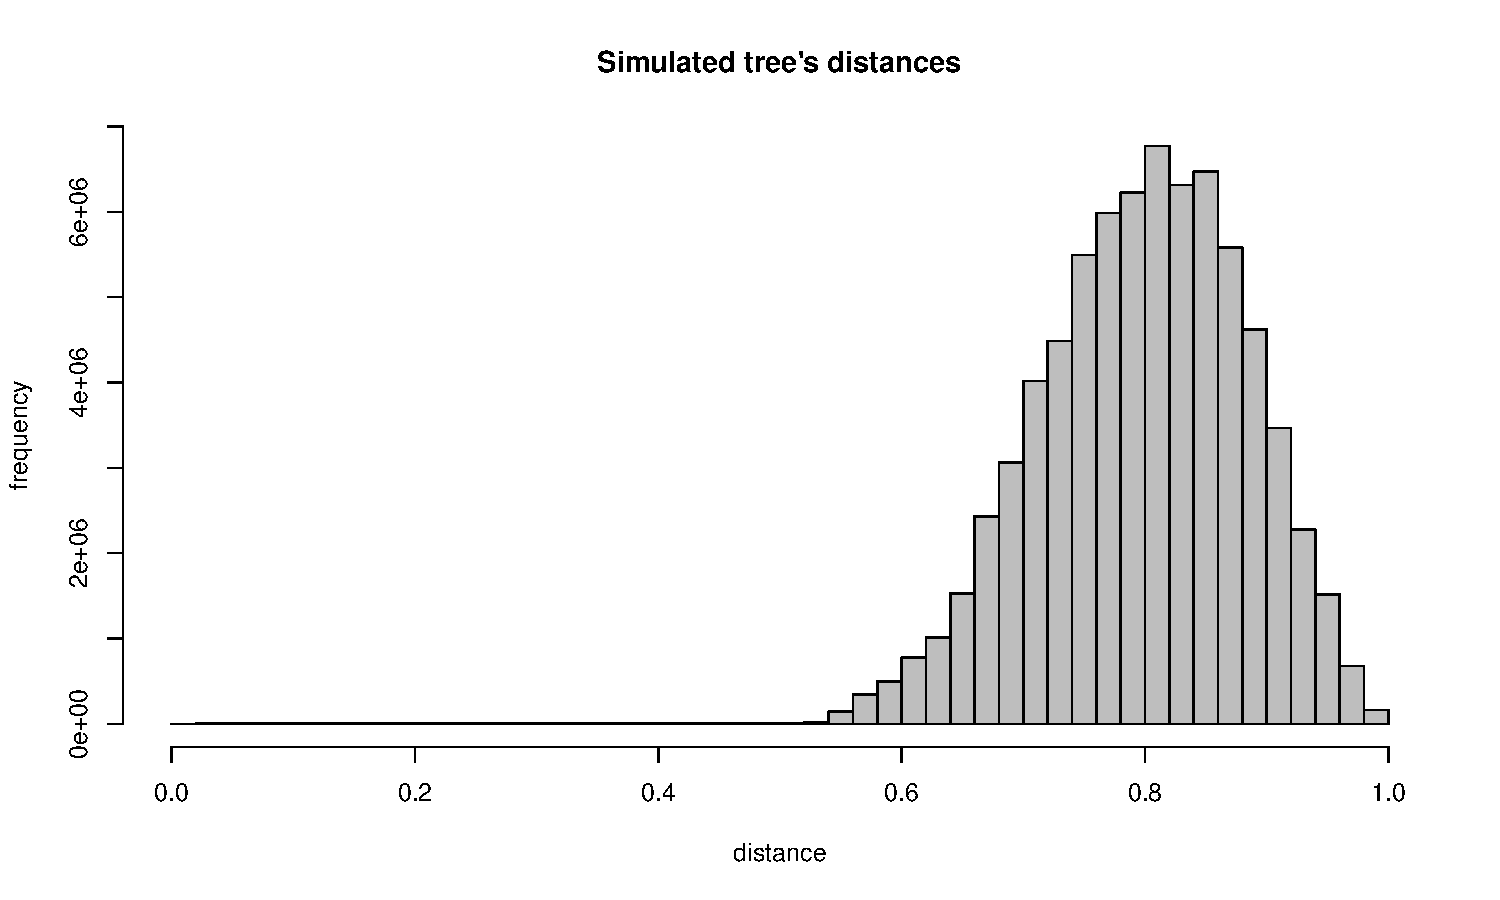
\includegraphics[width=10cm]{figure/plotget_distances-1} 
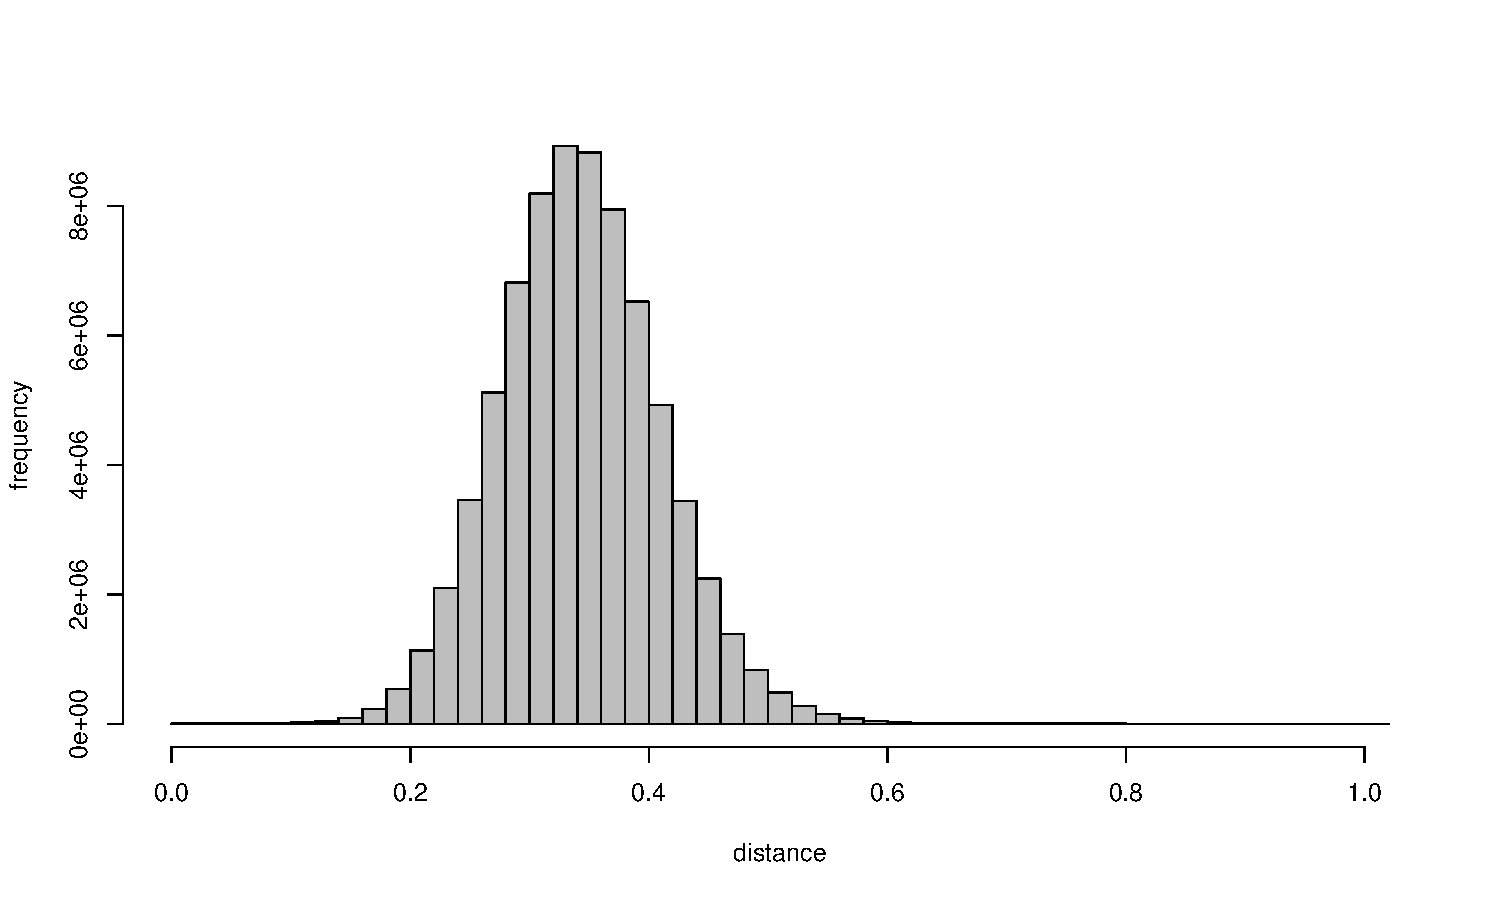
\includegraphics[width=10cm]{figure/plotget_distances-2} 

}



\end{knitrout}

\section{Clustering}
Clustering with fixed number of groups ?
\begin{knitrout}
\definecolor{shadecolor}{rgb}{0.969, 0.969, 0.969}\color{fgcolor}\begin{kframe}
\begin{alltt}
\hlstd{simhc} \hlkwb{<-} \hlkwd{hclust}\hlstd{(simx,} \hlkwc{method} \hlstd{=} \hlstr{"average"}\hlstd{)} \hlcom{# UPGMA}
\hlstd{ukhc} \hlkwb{<-} \hlkwd{hclust}\hlstd{(ukx,} \hlkwc{method} \hlstd{=} \hlstr{"average"}\hlstd{)}

\hlcom{##- cut based on height}
\hlkwa{if} \hlstd{(F)\{}
\hlcom{#- function of heights}
\hlstd{nheights} \hlkwb{<-} \hlnum{10} \hlcom{# number of threshold}
\hlstd{up} \hlkwb{<-} \hlkwd{round}\hlstd{(}\hlkwd{mean}\hlstd{(simx),} \hlnum{1}\hlstd{)} \hlcom{# cut up to the mean}
\hlcom{# breaks <-  seq(1/nbreaks, 1-(1/nbreaks), by = 1/nbreaks)}
\hlstd{simclus} \hlkwb{<-} \hlkwd{cutree}\hlstd{(simhc,} \hlkwc{h} \hlstd{=} \hlkwd{seq}\hlstd{(up} \hlopt{/} \hlstd{nheights, up,} \hlkwc{by} \hlstd{= up} \hlopt{/} \hlstd{nheights) )} \hlcom{# h = breaks}
\hlstd{up} \hlkwb{<-} \hlkwd{round}\hlstd{(}\hlkwd{mean}\hlstd{(ukx),}\hlnum{1}\hlstd{)} \hlcom{# cut up to the mean}
\hlstd{ukclus} \hlkwb{<-} \hlkwd{cutree}\hlstd{(ukhc,}  \hlkwc{h} \hlstd{=} \hlkwd{seq}\hlstd{(up} \hlopt{/} \hlstd{nheights, up,} \hlkwc{by} \hlstd{= up} \hlopt{/}\hlstd{nheights) )}
\hlcom{# rm(simx, ukx)}
\hlstd{\}}

\hlcom{#- cut as function of k groups}
\hlstd{kgroups} \hlkwb{<-} \hlkwd{c}\hlstd{(}\hlnum{500}\hlstd{,} \hlnum{1000}\hlstd{,} \hlnum{5000}\hlstd{,} \hlnum{8000}\hlstd{,} \hlnum{10000}\hlstd{)}
\hlstd{simclus} \hlkwb{<-} \hlkwd{cutree}\hlstd{(simhc,} \hlkwc{k} \hlstd{= kgroups )} \hlcom{# h = breaks}
\hlstd{ukclus} \hlkwb{<-} \hlkwd{cutree}\hlstd{(ukhc,}  \hlkwc{k} \hlstd{= kgroups )}
\hlcom{# colnames(simclus) <- paste("k",colnames(simclus),sep='')}
\hlcom{# colnames(ukclus) <- paste("k",colnames(ukclus),sep='')}
\hlkwd{head}\hlstd{(simclus)}
\end{alltt}
\begin{verbatim}
   500 1000 5000 8000 10000
7    1    1    1    1     1
8    2    2    2    2     2
9    3    3    3    3     3
10   4    4    4    4     4
11   5    5    5    5     5
12   6    6    6    6     6
\end{verbatim}
\begin{alltt}
\hlkwd{head}\hlstd{(ukclus)}
\end{alltt}
\begin{verbatim}
      500 1000 5000 8000 10000
34695   1    1    1    1     1
21677   1    1    1    1     1
72292   1    1    2    2     2
81292   1    1    1    3     3
85197   1    1    3    4     4
53538   1    1    4    5     5
\end{verbatim}
\begin{alltt}
\hlcom{##- Calculate size(=Freq) of each cluster across different threshold}
\hlstd{simfreqClust} \hlkwb{<-} \hlkwd{apply}\hlstd{(simclus,} \hlnum{2}\hlstd{,} \hlkwa{function}\hlstd{(}\hlkwc{x}\hlstd{)} \hlkwd{as.data.frame}\hlstd{(}\hlkwd{table}\hlstd{(x)))} \hlcom{# list}
\hlstd{ukfreqClust} \hlkwb{<-} \hlkwd{apply}\hlstd{(ukclus,} \hlnum{2}\hlstd{,} \hlkwa{function}\hlstd{(}\hlkwc{x}\hlstd{)} \hlkwd{as.data.frame}\hlstd{(}\hlkwd{table}\hlstd{(x)))}
\hlcom{# str(simfreqClust)}
\hlcom{# head(simfreqClust[[1]])}

\hlcom{##- number of different clusters by threshold # if number varies !}
\hlcom{# sapply(simfreqClust, function(x) dim(x)[1])}
\hlcom{# sapply(ukfreqClust, function(x) dim(x)[1])}

\hlcom{##- cluster size}
\hlcom{#- sim}
\hlkwd{sapply}\hlstd{(simfreqClust,} \hlkwa{function}\hlstd{(}\hlkwc{x}\hlstd{)} \hlkwd{summary}\hlstd{(x}\hlopt{$}\hlstd{Freq))}
\end{alltt}
\begin{verbatim}
            500    1000   5000  8000 10000
Min.       1.00    1.00  1.000  1.00 1.000
1st Qu.    2.00    2.00  1.000  1.00 1.000
Median     6.00    6.00  2.000  1.00 1.000
Mean      24.33   12.16  2.433  1.52 1.216
3rd Qu.   13.00   13.00  3.000  2.00 1.000
Max.    7395.00 3019.00 20.000 11.00 7.000
\end{verbatim}
\begin{alltt}
\hlcom{#- uk}
\hlkwd{sapply}\hlstd{(ukfreqClust,} \hlkwa{function}\hlstd{(}\hlkwc{x}\hlstd{)} \hlkwd{summary}\hlstd{(x}\hlopt{$}\hlstd{Freq))}
\end{alltt}
\begin{verbatim}
            500    1000    5000  8000  10000
Min.       1.00    1.00   1.000  1.00  1.000
1st Qu.    1.00    1.00   1.000  1.00  1.000
Median     2.00    2.00   1.000  1.00  1.000
Mean      24.33   12.16   2.433  1.52  1.216
3rd Qu.    7.00    6.00   2.000  1.00  1.000
Max.    6868.00 3486.00 142.000 86.00 39.000
\end{verbatim}
\begin{alltt}
\hlcom{##- percentiles}
\hlcom{# sapply(freqClust, function(x) round(quantile(x$Freq, }
\hlcom{# probs = c(0.01, 0.05, 0.1, 0.25, 0.5, 0.75, 0.95, 0.99, 1))))}
\hlcom{# }
\end{alltt}
\end{kframe}
\end{knitrout}

Distribution of sizes - untransformed, transformed
\begin{knitrout}
\definecolor{shadecolor}{rgb}{0.969, 0.969, 0.969}\color{fgcolor}\begin{kframe}
\begin{alltt}
\hlcom{##- distr of cluster sizes: log(x) and Y untransformed}
\hlkwd{par}\hlstd{(}\hlkwc{mfcol}\hlstd{=}\hlkwd{c}\hlstd{(}\hlnum{2}\hlstd{,} \hlkwd{length}\hlstd{(kgroups)))}
\hlkwa{for} \hlstd{(i} \hlkwa{in} \hlnum{1}\hlopt{:}\hlkwd{length}\hlstd{(kgroups))\{}
  \hlstd{h} \hlkwb{<-} \hlkwd{hist}\hlstd{(}\hlkwd{log}\hlstd{(ukfreqClust[[i]]}\hlopt{$}\hlstd{Freq),}
       \hlkwc{main} \hlstd{=} \hlkwd{paste}\hlstd{(}\hlstr{"uk"}\hlstd{,} \hlkwd{names}\hlstd{(ukfreqClust)[i]),}
       \hlkwc{xlab} \hlstd{=} \hlstr{"log(size)"}\hlstd{)}
  \hlkwd{hist}\hlstd{(}\hlkwd{log}\hlstd{(simfreqClust[[i]]}\hlopt{$}\hlstd{Freq),}
       \hlkwc{main} \hlstd{=} \hlkwd{paste}\hlstd{(}\hlstr{"sim"}\hlstd{,} \hlkwd{names}\hlstd{(simfreqClust)[i]),}
       \hlkwc{xlab} \hlstd{=} \hlstr{"log(size)"}\hlstd{)}
\hlstd{\}}

\hlcom{##- distr of cluster sizes: log(x) and log(y)}
\hlkwd{par}\hlstd{(}\hlkwc{mfcol}\hlstd{=}\hlkwd{c}\hlstd{(}\hlnum{2}\hlstd{,} \hlkwd{length}\hlstd{(kgroups)))}
\hlkwa{for} \hlstd{(i} \hlkwa{in} \hlnum{1}\hlopt{:}\hlkwd{length}\hlstd{(kgroups))\{}
  \hlstd{h} \hlkwb{<-} \hlkwd{hist}\hlstd{(}\hlkwd{log}\hlstd{(ukfreqClust[[i]]}\hlopt{$}\hlstd{Freq),} \hlkwc{plot} \hlstd{= F)}
  \hlstd{h}\hlopt{$}\hlstd{counts} \hlkwb{<-} \hlkwd{log1p}\hlstd{(h}\hlopt{$}\hlstd{counts)} \hlcom{# log(y)}
  \hlkwd{plot}\hlstd{(h,} \hlkwc{ylab} \hlstd{=} \hlstr{"log(Freq)"}\hlstd{,}
       \hlkwc{main} \hlstd{=} \hlkwd{paste}\hlstd{(}\hlstr{"uk"}\hlstd{,} \hlkwd{names}\hlstd{(ukfreqClust)[i]),}
       \hlkwc{xlab} \hlstd{=} \hlstr{"log(size)"}\hlstd{)}

  \hlstd{h} \hlkwb{<-} \hlkwd{hist}\hlstd{(}\hlkwd{log}\hlstd{(simfreqClust[[i]]}\hlopt{$}\hlstd{Freq),} \hlkwc{plot} \hlstd{= F)}
  \hlstd{h}\hlopt{$}\hlstd{counts} \hlkwb{<-} \hlkwd{log1p}\hlstd{(h}\hlopt{$}\hlstd{counts)} \hlcom{# log(y)}
  \hlkwd{plot}\hlstd{(h,} \hlkwc{ylab} \hlstd{=} \hlstr{"log(Freq)"}\hlstd{,}
          \hlkwc{main} \hlstd{=} \hlkwd{paste}\hlstd{(}\hlstr{"sim"}\hlstd{,} \hlkwd{names}\hlstd{(simfreqClust)[i]),}
          \hlkwc{xlab} \hlstd{=} \hlstr{"log(size)"}\hlstd{)}

\hlstd{\}}
\end{alltt}
\end{kframe}

{\centering 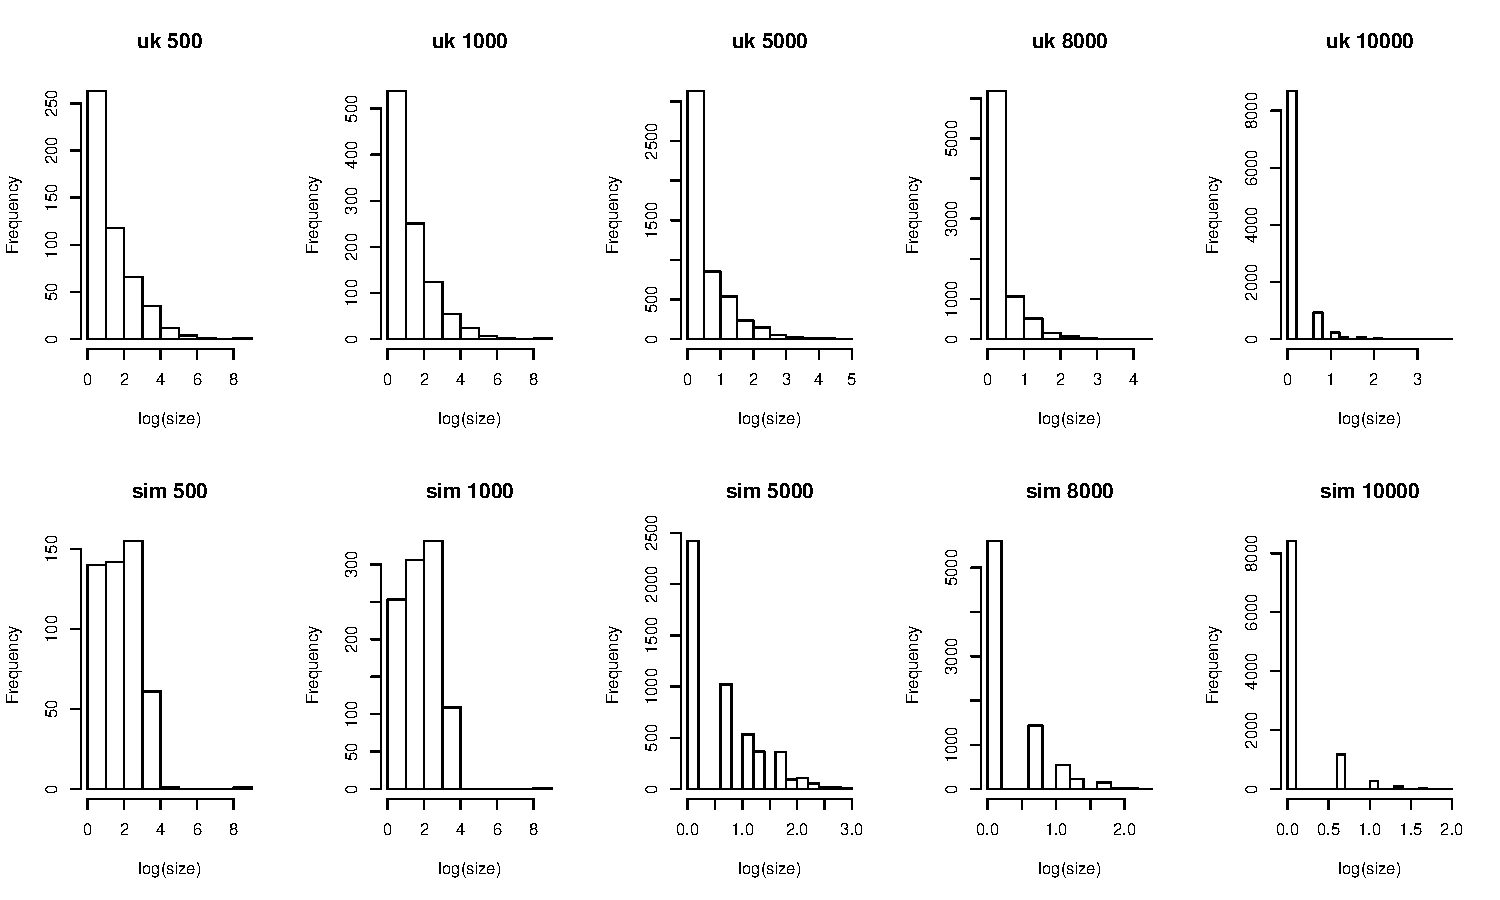
\includegraphics[width=10cm]{figure/plotplot_cluster_size-1} 
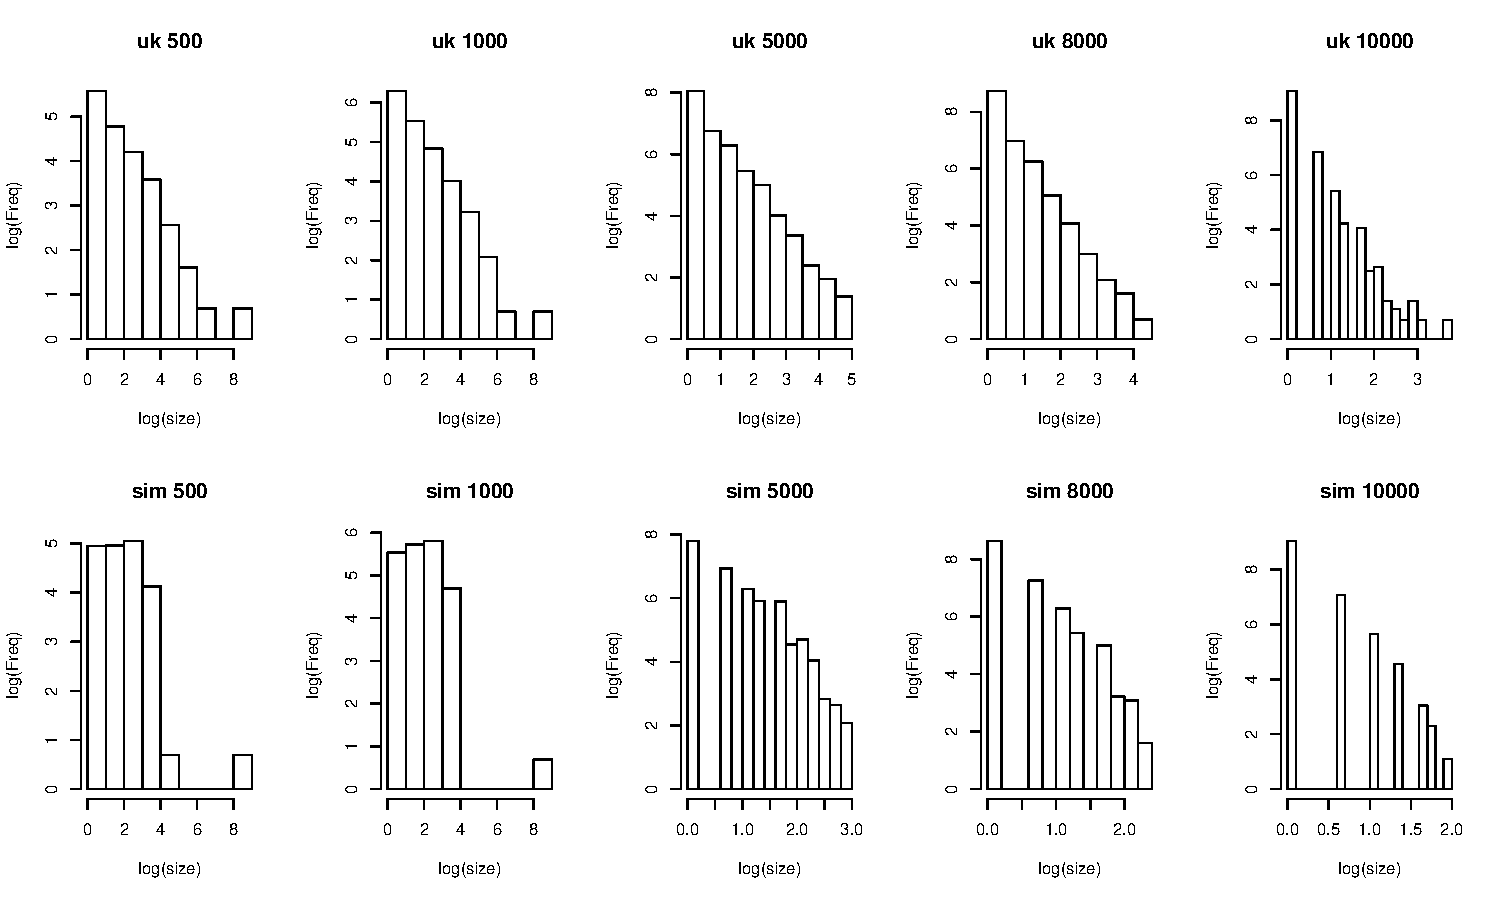
\includegraphics[width=10cm]{figure/plotplot_cluster_size-2} 

}



\end{knitrout}

QQ plot
\begin{knitrout}
\definecolor{shadecolor}{rgb}{0.969, 0.969, 0.969}\color{fgcolor}\begin{kframe}
\begin{alltt}
\hlkwd{par}\hlstd{(}\hlkwc{mfcol}\hlstd{=}\hlkwd{c}\hlstd{(}\hlnum{2}\hlstd{,} \hlkwd{length}\hlstd{(kgroups)))}
\hlkwa{for} \hlstd{(i} \hlkwa{in} \hlnum{1}\hlopt{:}\hlkwd{length}\hlstd{(kgroups))\{}
  \hlkwd{qqplot}\hlstd{(ukfreqClust[[i]]}\hlopt{$}\hlstd{Freq,}
         \hlstd{simfreqClust[[i]]}\hlopt{$}\hlstd{Freq,}
         \hlkwc{main} \hlstd{=} \hlkwd{names}\hlstd{(ukfreqClust)[i],}
         \hlkwc{xlab} \hlstd{=} \hlstr{"uk"}\hlstd{,} \hlkwc{ylab} \hlstd{=} \hlstr{"sim"}\hlstd{)}

  \hlkwd{qqplot}\hlstd{(}\hlkwd{log}\hlstd{(ukfreqClust[[i]]}\hlopt{$}\hlstd{Freq),}
         \hlkwd{log}\hlstd{(simfreqClust[[i]]}\hlopt{$}\hlstd{Freq),}
         \hlkwc{main} \hlstd{=} \hlkwd{names}\hlstd{(ukfreqClust)[i],}
         \hlkwc{xlab} \hlstd{=} \hlstr{"log(uk)"}\hlstd{,} \hlkwc{ylab} \hlstd{=} \hlstr{"log(sim)"}\hlstd{)}

\hlstd{\}}
\end{alltt}
\end{kframe}

{\centering 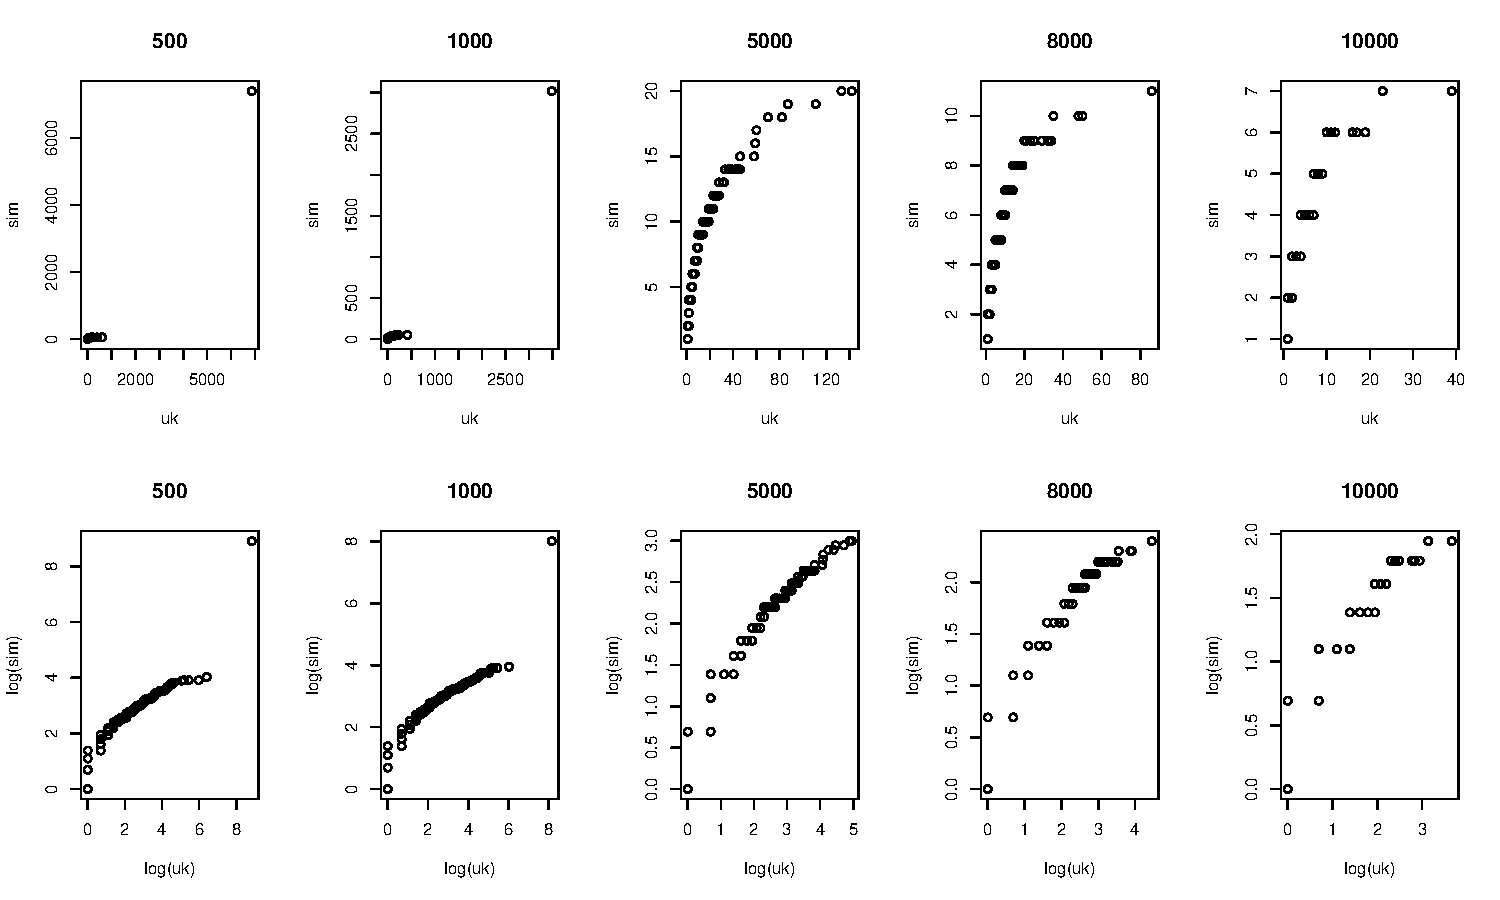
\includegraphics[width=10cm]{figure/plotQQ_plot-1} 

}



\end{knitrout}
% ggplot unecessary

\section{Add patients data}
Add data from sample states and time
\begin{knitrout}
\definecolor{shadecolor}{rgb}{0.969, 0.969, 0.969}\color{fgcolor}\begin{kframe}
\begin{alltt}
\hlcom{##- converting sample states in table of co-variates ?}
\hlstd{demes} \hlkwb{<-} \hlkwd{as.vector}\hlstd{(}\hlkwd{read.csv}\hlstd{(}\hlkwc{file} \hlstd{=} \hlstr{"demes.csv"}\hlstd{)}\hlopt{$}\hlstd{x)}
\hlstd{sampleTimes} \hlkwb{<-} \hlkwd{scan}\hlstd{(} \hlkwc{file} \hlstd{=} \hlstr{'sampleTimes'} \hlstd{)}
\hlstd{ss}  \hlkwb{<-} \hlkwd{matrix}\hlstd{(} \hlkwd{scan}\hlstd{(} \hlkwc{file} \hlstd{=} \hlstr{'sampleStates'} \hlstd{) ,}
               \hlkwc{byrow} \hlstd{=} \hlnum{TRUE}\hlstd{,}
               \hlkwc{ncol} \hlstd{=} \hlkwd{length}\hlstd{(demes))}
\hlkwd{colnames}\hlstd{(ss)} \hlkwb{<-} \hlstd{demes}
\hlkwd{dim}\hlstd{(ss)}
\end{alltt}
\begin{verbatim}
[1] 12164   121
\end{verbatim}
\begin{alltt}
\hlkwd{max}\hlstd{(ss[,}\hlnum{121}\hlstd{])} \hlcom{# nothing on source}
\end{alltt}
\begin{verbatim}
[1] 0
\end{verbatim}
\begin{alltt}
\hlstd{demo} \hlkwb{<-} \hlkwd{data.frame}\hlstd{()}
\hlkwa{for} \hlstd{(i} \hlkwa{in} \hlnum{1}\hlopt{:}\hlkwd{dim}\hlstd{(ss)[}\hlnum{1}\hlstd{])\{} \hlcom{# dim(ss)[1]}
  \hlstd{deme} \hlkwb{<-} \hlkwd{names}\hlstd{(}\hlkwd{which}\hlstd{(ss[i,]} \hlopt{==} \hlnum{1}\hlstd{))} \hlcom{# name of column which has value 1}
  \hlstd{patient} \hlkwb{<-} \hlstd{i}
  \hlstd{time} \hlkwb{<-} \hlstd{sampleTimes[i]}
  \hlstd{age} \hlkwb{<-} \hlkwd{as.numeric}\hlstd{(} \hlkwd{regmatches}\hlstd{( deme,}
                \hlkwd{regexec}\hlstd{(} \hlstr{"\textbackslash{}\textbackslash{}.age([0-9])"}\hlstd{, deme) )[[}\hlnum{1}\hlstd{]][}\hlnum{2}\hlstd{] )}
  \hlstd{care} \hlkwb{<-} \hlkwd{as.numeric}\hlstd{(} \hlkwd{regmatches}\hlstd{( deme,}
                \hlkwd{regexec}\hlstd{(} \hlstr{"care([0-9])"}\hlstd{, deme) )[[}\hlnum{1}\hlstd{]][}\hlnum{2}\hlstd{] )}
  \hlstd{stage} \hlkwb{<-} \hlkwd{as.numeric}\hlstd{(} \hlkwd{regmatches}\hlstd{( deme,}
                \hlkwd{regexec}\hlstd{(} \hlstr{"stage([0-9])"}\hlstd{, deme) )[[}\hlnum{1}\hlstd{]][}\hlnum{2}\hlstd{] )}
  \hlstd{risk} \hlkwb{<-} \hlkwd{as.numeric}\hlstd{(} \hlkwd{regmatches}\hlstd{( deme,}
                \hlkwd{regexec}\hlstd{(} \hlstr{"riskLevel([0-9])"}\hlstd{, deme) )[[}\hlnum{1}\hlstd{]][}\hlnum{2}\hlstd{] )}
  \hlstd{demo} \hlkwb{<-} \hlkwd{rbind}\hlstd{(demo,} \hlkwd{cbind}\hlstd{(}
    \hlstd{patient, time, age, care, stage, risk))}
\hlstd{\}}
\hlkwd{str}\hlstd{(demo)}
\end{alltt}
\begin{verbatim}
'data.frame':	12164 obs. of  6 variables:
 $ patient: num  1 2 3 4 5 6 7 8 9 10 ...
 $ time   : num  11245 8627 6679 8446 8900 ...
 $ age    : num  3 3 4 4 4 3 4 3 3 4 ...
 $ care   : num  1 1 1 1 1 1 1 1 1 1 ...
 $ stage  : num  1 1 1 5 4 2 5 2 3 5 ...
 $ risk   : num  1 1 1 1 1 1 1 1 2 1 ...
\end{verbatim}
\begin{alltt}
\hlcom{##- date of diagnosis ?}
\hlstd{date0} \hlkwb{<-} \hlkwd{as.Date}\hlstd{(}\hlstr{'1979-01-01'}\hlstd{)}
\hlstd{demo}\hlopt{$}\hlstd{datediag} \hlkwb{<-} \hlstd{date0} \hlopt{+} \hlstd{demo}\hlopt{$}\hlstd{time}
\hlkwd{min}\hlstd{(demo}\hlopt{$}\hlstd{datediag)}
\end{alltt}
\begin{verbatim}
[1] "1996-11-15"
\end{verbatim}
\begin{alltt}
\hlkwd{max}\hlstd{(demo}\hlopt{$}\hlstd{datediag)}
\end{alltt}
\begin{verbatim}
[1] "2013-02-15"
\end{verbatim}
\end{kframe}
\end{knitrout}

Add cluster size by patient
\begin{knitrout}
\definecolor{shadecolor}{rgb}{0.969, 0.969, 0.969}\color{fgcolor}\begin{kframe}
\begin{alltt}
\hlcom{####... and outdegrees}
\end{alltt}
\end{kframe}
\end{knitrout}





\end{document}
